\documentclass{amsart}
\usepackage[foot]{amsaddr} % put addresses on first page

\usepackage{geometry}
\usepackage{booktabs}
\usepackage{graphicx,psfrag,epsf}
\usepackage{enumerate}
\usepackage{enumitem}
\usepackage{amsfonts}
\usepackage{mathtools}
\usepackage{amssymb}
\usepackage{amsmath}
\allowdisplaybreaks
\usepackage{longtable}
\usepackage{bigints}
\usepackage{siunitx}
\usepackage{algpseudocode}
\usepackage{algorithm}
\usepackage{amsthm}
\usepackage{soul}
\usepackage{color}

\usepackage{hyperref}
\usepackage[capitalise]{cleveref}
\newtheorem{theorem}{Theorem}[section]
\newtheorem{corollary}{Corollary}[theorem]
\newtheorem{lemma}{Lemma}[theorem]
\newtheorem{definition}{Definition}[section]
%

\usepackage[numbers]{natbib}
\usepackage{url} % not crucial - just used below for the URL 
\usepackage{doi}

\title{Copula estimation using loss-based Bayesian Additive Regression Trees}
\author{**}
\date{\today}

\begin{document}

\maketitle

\section{Introduction}

\section{Model}

\subsection{Conditional copula}

Copulas are extremely useful  for modelling the dependence structure between random variables when we wish to separate the marginals from their joint distribution. \citet{sklar:1959} showed the existence of such unique copulas $C:[0,1]^p\to [0,1]$ such that
\begin{equation*}
	H(Y_1,Y_2,\cdots, Y_p) = C(F_1(Y_1),F_2(Y_2),\cdots,F_p(Y_p)).
\end{equation*}
In some cases, there might be additional confounding random variable $X$ that influences the dependence between $Y_1,Y_2,\cdots, Y_p$. 

In such cases, a conditional copula is used to understand the dependence structure. A conditional copula was first formalised by \citet{patton2006}. For simplicity we present the formulation for two variables. Let $Y_1$ and $Y_2$ be two continuous random variables and $X$ be a continuous random variable that might affect the relationship between $Y_1$ and $Y_2$. Then according to Sklar’s theorem there exists a unique copula such that:
\begin{equation*}
    H(Y_1,Y_2\mid X) = C_X(F_{1X}(Y_1\mid X),F_{1X}(Y_2\mid X)); \quad \forall (y_1,y_2) \in \mathbb{R}^2
\end{equation*}
where $C_X \coloneqq C(\cdot\mid \theta(X))$ is the copula function that varies with respect to $X$ through the copula parameter $\theta$ and $F_{iX}(Y_i\mid X)$ is the cdf of $Y_i$ conditional on $X$ for $i=1,2$.

This gives us the following copula distribution function
\begin{equation*}
    C_X(u_1,u_2) = H\left(F_{1X}^{-1}(Y_1\mid X),F_{2X}^{-1}(Y_2\mid X)\mid X\right)
\end{equation*}
where $u_k = F_{1X}(Y_k\mid X)$ for $i=1,2$.

\subsection{Loss-based BART}

Let, $Z$ be an outcome data such that 
\begin{equation*}
	Z_i \sim \mathcal{N}\left(r(x_i),\sigma^2\right);\qquad 1\le i\le n.
\end{equation*}
Then we can approximate this function $r(x)$ with sum of regression trees such such that,
\begin{equation*}
	r(x_i) = \sum_{t=1}^m g(x_i, T_t, M_t).
\end{equation*}
where $T_t$ denotes the $t$-th tree, $M_t$ denotes the vector of terminal node values $M_t = \{\mu_1,\mu_2, \cdots, \mu_{n_L(T_t)}\}$ of the $t$-th tree and $n_L(T_t)$ denotes the number of terminal nodes of the $t$-th tree. 

Recently, \citet{serafini2024lossbasedpriortreetopologies} proposed a loss-based prior for BART in the following way:
\begin{align}
	\begin{split}
	    T_t, M_t &\sim \pi(T_t)\pi(M_t\mid T_t)\\
	T_t &\propto \exp\left(\omega n_L(T_t)-\gamma\Delta(T_t)\right)\\
	\pi(M_t\mid T_t) & = \prod_{j=1}^{n_L(T_t)}\pi(\mu_j\mid T_t).
	\end{split}
\end{align}
where $\Delta(T_t)$ is the difference between right terminal nodes and left terminal nodes of $t$-th given tree.

For the choice of prior on $\mu_j\mid T_t$ \citet{chipman_BART,serafini2024lossbasedpriortreetopologies} suggested a conjugate prior with respect to the likelihood function. 

\subsection{Copula Parameter Estimation}

We wish to employ this loss-based prior for BART for the estimation of $\theta(x)$. Let $c(u_1,u_2\mid \theta(x))$ denote the conditional copula density function. Then we can define the following hierarchical model
\begin{align}
	\begin{split}
	    u_{1i},u_{2i} \mid \theta(x_i) & \sim c(u_{1i},u_{2i}\mid \sum_{t=1}^m g(x_i, T_t, M_t))\\
	T_t &\propto \exp\left(\omega n_L(T_t)-\gamma\Delta(T_t)\right)\\
	\pi(M_t\mid T_t) &\propto \prod_{j=1}^{n_L(T_t)}\pi(\mu_j\mid T_t)\\
	t & = 1,2,\cdots m.
	\end{split}
\end{align}

This gives us the following posterior:
\begin{equation}
	\pi(T,M \mid U_1, U_2, X) \propto \prod_{i=1}^{n}c\left(u_{1i},u_{2i}\mid \sum_{t=1}^m g(x_i, T_t, M_t)\right)\prod_{t=1}^{m}\pi(T_t)\prod_{t=1}^{m}\pi(M_t\mid T_t).
\end{equation}

To sample from the posterior we use backfitting algorithm where we sample $(T_j, M_j)$ conditional on the other $m-1$ pairs of $(T_k,M_k)$. Therefore, we define $R_{ij}$ such that
\begin{equation*}
	R_{ij} = \sum_{t\not=j}g(x_i, T_t, M_t)
\end{equation*}
Then the posterior of $j$-th pair conditional on $R_j$ is given by:
\begin{align}\label{eq:post:res}
	\begin{split}
	    \pi(T_j,M_j \mid R_j, U_1,U_2 X) &\propto \prod_{i=1}^{n}c\left(u_{1},u_{2}\mid R_j+g(x, T_j, M_j)\right)\pi(T_j)\pi(M_j\mid T_j)\\
	&\propto \pi(T_j)\prod_{i=1}^{n}c\left(u_{1},u_{2}\mid R_j+g(x, T_j, M_j)\right)\prod_{k=1}^{n_L(T_j)}\pi(\mu_k\mid T_j)
	\end{split}
\end{align}

\section{MCMC for Parameter Estimation}
For standard BART model, the use of conjugate prior allows us to marginalise the likelihood with respect to $\mu_j$ such that:
\begin{equation}
	\mathcal{L}(U_1,U_2\mid X, T)\propto \bigint_{\mu}\left(\prod_{i=1}^{n}c\left(u_{1},u_{2}\mid R_j+g(x, T_j, M_j)\right)\prod_{k=1}^{n_L(T_j)}\pi(\mu_k\mid T_j)\right)d\mu.
\end{equation}

Unfortunately, we do not have the conjugacy property in our case. So we use a Metropolis Hastings algorithm to compute from the posterior given by \cref{eq:post:res}.

For that, we first choose a proposal distribution, $q\left(T_t^k,M_t^k;T_t^\ast, M_t^\ast\right)$ to generate a proposal at the $k$-th step.

\begin{align}\label{eq:prop}
	q\left(T_t^k,M_t^k;T_t^\ast, M_t^\ast\right) = q\left(T_t^k;T_t^\ast\right) q\left(M_t^k;T_t^k, T_t^\ast, M_t^\ast\right).
\end{align}

\subsection{proposal for tree}
For $q\left(T_t^k;T_t^\ast\right)$ we follow the steps given by \citet{serafini2024lossbasedpriortreetopologies}. 

\begin{itemize}
	\item \textsc{grow}: Randomly choose a terminal node and split it into two terminal nodes
	\item \textsc{prune}: Randomly choose a parent of terminal nodes and turn into a terminal node
	\item \textsc{change}: Randomly choose an internal node and assign a new splitting rule
    \item \textsc{swap}: Randomly choose a parent-child pair of internal node and swap their splitting rules
\end{itemize}

The moves are performed to ensure that $T_t^\ast$ yields a valid partition defined as followed.

\begin{definition}[Cell size] Given a $\mathbf{\Omega} = \{\Omega_k\}_{k=1}^N$ of $\mathcal{X} = [0,1]$ and a set of observations $x_1, x_2, \cdots, x_n$ such that $x_i\in \mathcal{X}$ for $i=1,2,\cdots, n$, the sell size $S(\Omega_k)$ of $\Omega_k$
is the fraction of observations contained in $\Omega_k$.
\begin{equation*}
    S(\Omega_k) = \frac{1}{n}\sum_{j=1}^n \mathbb{I}(x_j\in \Omega_k).
\end{equation*}
\end{definition}

\begin{definition}[Valid partition]
    A partition is said to be valid if
    \begin{equation*}
        S(\Omega_k) \ge \frac{C^2}{n}, \quad\text{for any } k=1,2,\cdots, N
    \end{equation*}
    for a constant $C^2\ge 1$.
\end{definition}

For $q\left(M_t^k;T_t^k, T_t^\ast, M_t^\ast\right)$ we generate new terminal node values based on the terminal node values of the previous tree.

For instance;

\begin{itemize}
	\item For \textsc{grow} we consider the $j$-th leaf to be grown so,
	$q\left(M_t^k;T_t^k, T_t^\ast, M_t^\ast\right)$ = $\pi_{prop}(\mu_j)*\pi_{prop}(\mu_j)$
	\item For \textsc{prune} we consider the $j$th and $(j+1)$th leaves to be pruned then $q\left(M_t^k;T_t^k, T_t^\ast, M_t^\ast\right)$ = $\pi_{prop}((\mu_j + \mu_{j+1})/2)$
	\item For \textsc{change} we consider the split condition will change the terminal node value of $j$th and $(j+1)$th leaves then $q\left(M_t^k;T_t^k, T_t^\ast, M_t^\ast\right)$ = $\pi_{prop}(\mu_j)*\pi_{prop}(\mu_{j+1})$
\end{itemize}

Using $q$, we calculate the acceptance probability such that
\begin{equation}\label{eq:acc:prob}
	\alpha\left(T_t^k,M_t^k;T_t^\ast, M_t^\ast\right)
	= \frac{\pi(T_t^\ast,M_t^\ast \mid R_t, U_1, U_2, X)q\left(T_t^\ast, M_t^\ast;T_t^k,M_t^k\right)}
	{\pi(T_t^k,M_t^k \mid R_t, U_1, U_2, X)q\left(T_t^k,M_t^k;T_t^\ast, M_t^\ast\right)}
\end{equation}

\begin{algorithm}
	\caption{One iteration of MCMC for copula BART}
	
	\begin{algorithmic}[1]
		\State The previous steps gives us $(T^k,M^k)$
		\State Set $\theta(x_i) \leftarrow \sum_{t=1}^{m} g(x_i, T^k_t, M^k_t)$ for $i = 1, \ldots, n$
		\For{$t = 1, \ldots, m$}
		\State Set $R_{it} \leftarrow \sum_{j\not=t}g(x_i, T_j^k, M_j^k)$ for $i = 1, \ldots, n$
		
		\State Sample $(T_t^\ast, M_t^\ast)$ using $q\left(T_t^k,M_t^k;T_t^\ast, M_t^\ast\right)$ in \cref{eq:prop} by randomly choosing between the \textsc{grow}, \textsc{prune}, \textsc{swap}, and \textsc{change} 
		
		\State Compute acceptance probability using $\alpha\left(T_t^k,M_t^k;T_t^\ast, M_t^\ast\right)$ in \cref{eq:acc:prob}.
		
		\State Set $(T_t^{k+1}, M_t^{k+1})=(T_t^\ast, M_t^\ast)$ with probability $\alpha\left(T_t^k,M_t^k;T_t^\ast, M_t^\ast\right)$ or $(T_t^{k+1}, M_t^{k+1})=(T_t^k,M_t^k)$.
		\State Set $\theta_i \leftarrow R_{it} + g(x_i T_t^{k+1}, M_t^{k+1})$ for $i = 1, \ldots, N$
		\EndFor
        \State Sample $M\coloneqq (M_1, M_2, \cdots, M_m)$ from the full conditional using MH step once all the new trees are formed.
	\end{algorithmic}
\end{algorithm}

\section{Simulation Studies}

To generate the true copula parameter, we first consider 4 different test cases to simulate Kendall's tau conditional on $x$. Such that

\begin{itemize}
	\item Case 1: True $\tau_x$ has a tree structure with respect to $x$. To obtain the tree structure we first generate a random binary tree such that number of terminal nodes is 8 and and difference between left and right terminal node is 4. Then we generate $\tau_x$ such that
	\begin{equation}
		\tau_x = \begin{cases}
			0.5 + \mathcal{N}(0,0.01) & x \le 0.25\\
			0.7 + \mathcal{N}(0,0.01) & 0.25 < x \le 0.6\\
			0.3 + \mathcal{N}(0,0.01) & 0.6 < x
		\end{cases}
	\end{equation}
	\item Case 2: True $\tau_x$ is monotone with respect to $x$ such that 
	\begin{equation}\label{eq:synth:tau_x:case2}
		\tau_x = 0.3 + 0.2 \sin(3x) + 0.3x^2.
	\end{equation}
	\item Case 3: True $\tau_x$ is convex with respect to $x$ such that 
	\begin{equation}\label{eq:synth:tau_x:case3}
		\tau_x = 0.5 + 0.3 \sin(3x).
	\end{equation}
	\item Case 4: True $\tau_x$ non-convex and non-monotone with respect to $x$ such that 
	\begin{equation}\label{eq:synth:tau_x:case4}
		\tau_x = 0.6 - 0.3 \sin(2x) + 0.2 \sin(4x) + 0.3 x^2.
	\end{equation}
\end{itemize}

We present the plot of true values of Kendall's $\tau$ with respect to $x$ in \cref{fig:true:tau}. Additionally, we provide the tree structure based $\tau_x$ in for clearer interpretation of the splitting rule.

\begin{figure}
	\centering
	\caption{Splitting rule for the tree based $\tau_x$}
	\label{fig:tau_tree_split}
	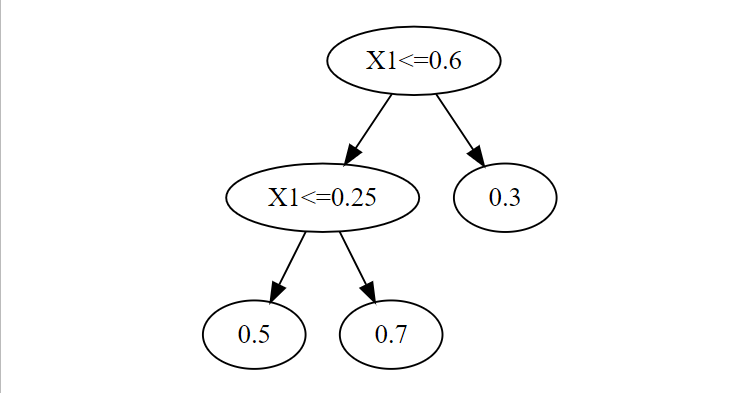
\includegraphics[width=0.5\linewidth]{tree_cond_tau_x.png}
\end{figure}

\begin{figure}
	\centering
	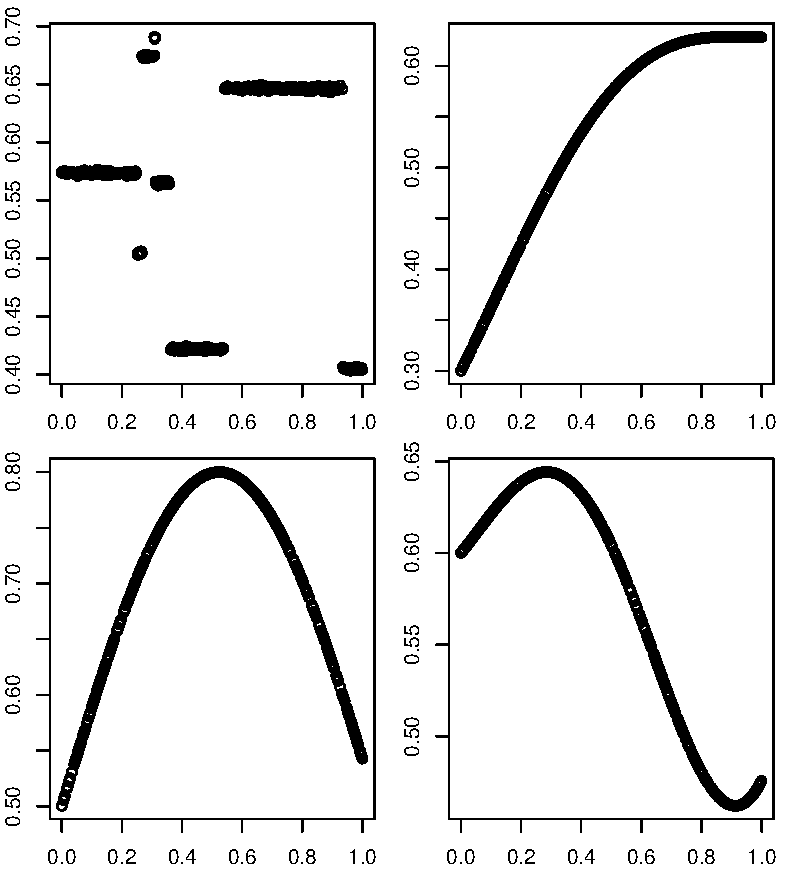
\includegraphics[width=0.95\linewidth]{true_tau.pdf}
	\caption{True values of Kendall's $\tau$ with respect to $x$. The top left plot shows case with tree structure; top right plot shows case defined by \cref{eq:synth:tau_x:case2}; bottom left shows case defined by \cref{eq:synth:tau_x:case3}; and bottom right shows case defined by \cref{eq:synth:tau_x:case4}.}
	\label{fig:true:tau}
\end{figure}

Then using these values of conditional Kendall's $\tau$, we generate the copula parameters using the link functions summarised in \cref{tab:cop:link}. Afterwards, we simulate from the copula density functions to obtain our synthetic dataset.

\begin{table}
	\centering
	\begin{tabular}{l|c|c|c}
		\toprule
		Family & Support & Relation with $\tau$ & Range of $\tau$ \\
		\midrule
		Gaussian & $\rho \in (-1,1)$ & $\sin(\tau\pi/2)$ & (-1,1)\\
		Student-t & $\rho \in (-1,1)$ & $\sin(\tau\pi/2)$ & (-1,1) \\
		Clayton & $\theta \in (0,\infty)$ & $2\tau/(1-\tau)$ & $(0,1)$ \\
		Gumbel & $\theta\in [1,\infty)$ & $1/(1-\tau)$  & $[0,1)$ \\
		\bottomrule
	\end{tabular}
	\caption{Copula families used for analyses, along with parameter support and relation with Kendall's $\tau$.}
	\label{tab:cop:link}
\end{table}

\paragraph{Prediction accuracy} For the sake of evaluating the efficiency of copula parameter estimation we check in sample prediction of the copula parameter ($\rho$ for Gaussian and student-t; $\theta$ for Clayton and Gumbel) using the posterior samples of the regression trees . 

There after we check the root mean squared error with respect to the true copula parameter used in the data generation phase. Given by:

\begin{equation}
	\text{RMSE} = \sqrt{\frac{1}{nC}\sum_{j=1}^C \sum_{i=1}^n (\theta_{i} - \overline{\theta}^*_{ij})^2}
\end{equation}
where $\overline{\theta}^*_i$ is posterior sample mean of copula parameter conditional on $x_i$ and $C$ is the total number of parallel chains.

For credible interval coverage, check whether the true copula parameter is contained within the 95\% credible interval of the predictive samples of the copula parameter

\begin{equation}
	\text{CI coverage} = \frac{\sum_{j=1}^C\sum_{i=1}^n\mathbb{I}\left(Q_{2.5}(\theta^*_{ij}) \le \theta_i \le Q_{97.5}(\theta^*_{ij})\right)}{nC}.
\end{equation}

Additionally, we check for credible interval length using $\frac{1}{nC}\left(Q_{97.5}(\theta^*_i) - Q_{2.5}(\theta^*_i)\right)$.

\subsection{Results}

\subsubsection{Choice of priors} For the Gaussian copula, the copula parameter $\rho$ lies within the open interval $(-1,1)$. So a natural choice for prior on $\mu_j$ is transformed beta as suggested by \citet{gokhale_prior_cor}. 

\begin{equation}
	\text{TBeta}(a, b) = \frac{1}{2^{a+b-1}\mathcal{B}(a,b)}(1+\rho)^{a-1}(1-\rho)^{b-1},
\end{equation}
for $a,b>0$ and $\mathcal{B}$ denotes beta function. 

For the student-t copula we are only interested in estimating $\rho$ which lies within $(-1,1)$. Therefore, similar to Gaussian copula, we use a transformed beta distribution as a prior on $\mu_j$. The copula parameter of the Clayton copula lies in the open interval $(0,\infty)$ and the copula parameter of the Gumbel copula lies in the open interval $[1,\infty)$. So we consider log-normal for $\mu_j$ for these two cases

We present the summary of our analyses with different copulas in \cref{tab:gauss:summary}. 

\begin{table}[ht]
	\centering
	\scriptsize{
	\begin{tabular}{ll|cccccc}
		\toprule
		& Prior on $\mu_j$ & $\mathbb{E}(n_L\mid U,X)$ & $\mathbb{E}(D\mid U,X)$ & Acc. Rate & RMSE & CI length & CI coverage \\ 
		\midrule
		\multicolumn{8}{c}{Gaussian} \\
		\midrule
		Case 1 & TBeta(1.1,1.1) & 6.4483 & 3.1417 & 0.2517 & 0.0143 & 0.4714 & 0.8200 \\ 
		Case 2 & TBeta(1.1,1.1) & 2.2783 & 1.2367 & 0.3050 & 0.0251 & 0.4621 & 0.7100 \\ 
		Case 3 & TBeta(1.1,1.1) & 3.4767 & 2.1433 & 0.3133 & 0.0057 & 0.2533 & 0.9700 \\ 
		Case 4 & TBeta(1.1,1.1) & 6.2267 & 3.7633 & 0.4450 & 0.0027 & 0.3062 & 1.0000 \\ 
		\midrule
		\multicolumn{8}{c}{Student t} \\
		\midrule
		Case 1 & TBeta(1.1,1.1) & 2.3733 & 1.2917 & 0.2283 & 0.0650 & 0.3692 & 0.2900 \\ 
		Case 2 & TBeta(1.1,1.1) & 2.2867 & 1.2333 & 0.3017 & 0.0086 & 0.3999 & 1.0000 \\ 
		Case 3 & TBeta(1.1,1.1) & 2.5483 & 1.4267 & 0.2400 & 0.0136 & 0.2842 & 1.0000 \\ 
		Case 4 & TBeta(1.1,1.1) & 2.2100 & 1.1800 & 0.3217 & 0.0084 & 0.4967 & 1.0000 \\ 
		\midrule
		\multicolumn{8}{c}{Clayton} \\
		\midrule
		Case 1 & LogNorm(0,1) & 2.2083 & 1.1817 & 0.1833 & 0.9492 & 1.9803 & 0.8200 \\ 
		Case 2 & LogNorm(0,1) & 2.2117 & 1.1767 & 0.4067 & 0.4144 & 2.0246 & 0.9500 \\ 
		Case 3 & LogNorm(0,1) & 2.1933 & 1.1583 & 0.1883 & 2.5465 & 3.0187 & 0.5800 \\ 
		Case 4 & LogNorm(0,1) & 2.2267 & 1.1933 & 0.3450 & 0.0706 & 2.4929 & 1.0000 \\
		\midrule
		\multicolumn{8}{c}{Gumbel} \\
		\midrule
		Case 1 & LogNorm(0,1) & 2.4317 & 1.3533 & 0.2150 & 0.2296 & 1.3673 & 0.8200 \\ 
		Case 2 & LogNorm(0,1) & 2.2917 & 1.2433 & 0.4267 & 0.0191 & 1.3536 & 1.0000 \\ 
		Case 3 & LogNorm(0,1) & 3.2050 & 1.8267 & 0.3850 & 0.4986 & 3.2591 & 1.0000 \\ 
		Case 4 & LogNorm(0,1) & 2.2883 & 1.2417 & 0.4533 & 0.1679 & 1.0935 & 0.9300 \\ 
		\bottomrule
		\end{tabular}}
	\caption{Summary of analyses with Gaussian copula. The columns represents the specific case, the type of prior on $\mu_j\mid T$, the posterior expected number of terminal nodes, the posterior expected depth, the acceptance rate of MH algorithm, RMSE of estimated $\rho$ against true $\rho$, length of credible interval and coverage frequency within the credible interval. The posterior quantities are obtained by running 100 different chains with 6000 samples in a single chain. We discard 1000 samples and then it is thinned by 10.}
	\label{tab:gauss:summary}
\end{table}

\paragraph{Convergence Diagnostic}
\begin{table}[ht]
	\centering
	\scriptsize{
		\begin{tabular}{ll|crr|crr|crr}
			\toprule
			\multicolumn{2}{c|}{} &
			\multicolumn{3}{c|}{Depth} &
			\multicolumn{3}{c|}{$n_L$} &
			\multicolumn{3}{c}{likelihood} \\
			\midrule
			& Prior & AC & ESS (\%) & Geweke & AC & ESS (\%) & Geweke & AC & ESS (\%) & Geweke \\ 
			\midrule
			\multicolumn{11}{c}{Gaussian} \\
			\midrule
			Case 1 & TBeta(1.1,1.1) & 0.90 & 0.14 & 0.50 & 0.96 & 0.13 & 0.53 & 0.25 & 2.44 & -0.64 \\ 
			Case 2 & TBeta(1.1,1.1) & 0.35 & 28.21 & 0.07 & 0.43 & 23.86 & -0.04 & 0.07 & 86.77 & -0.35 \\ 
			Case 3 & TBeta(1.1,1.1) & 0.45 & 13.17 & 0.36 & 0.45 & 15.06 & 0.00 & 0.41 & 24.98 & -1.03 \\ 
			Case 4 & TBeta(1.1,1.1) & 0.82 & 0.16 & 0.52 & 0.88 & 0.22 & 0.58 & 0.23 & 24.95 & 1.78 \\ 
			\midrule
			\multicolumn{11}{c}{Student t} \\
			\midrule
			Case 1 & TBeta(1.1,1.1) & 0.39 & 23.59 & 0.63 & 0.46 & 20.34 & 0.66 & 0.27 & 22.44 & 0.50 \\ 
			Case 2 & TBeta(1.1,1.1) & 0.25 & 48.89 & 0.24 & 0.34 & 42.33 & 0.46 & 0.15 & 71.96 & 0.29 \\ 
			Case 3 & TBeta(1.1,1.1) & 0.62 & 5.08 & -2.08 & 0.65 & 5.75 & -2.05 & 0.50 & 9.51 & 3.10 \\ 
			Case 4 & TBeta(1.1,1.1) & 0.43 & 15.35 & -1.74 & 0.51 & 12.34 & -2.09 & 0.64 & 5.05 & -2.31 \\ 
			\midrule
			\multicolumn{11}{c}{Clayton} \\
			\midrule
			Case 1 & LogNorm(0,1) & 0.26 & 16.98 & 0.82 & 0.33 & 16.91 & 0.96 & 0.22 & 37.78 & -1.51 \\ 
			Case 2 & LogNorm(0,1) & 0.24 & 62.78 & -0.86 & 0.33 & 49.50 & -1.00 & 0.44 & 21.32 & 1.19 \\ 
			Case 3 & LogNorm(0,1) & 0.23 & 24.41 & -2.09 & 0.30 & 18.37 & -2.28 & 0.68 & 17.24 & 0.50 \\ 
			Case 4 & LogNorm(0,1) & 0.18 & 79.41 & 0.01 & 0.23 & 75.73 & 0.21 & 0.38 & 27.08 & 0.36 \\ 
			\midrule
			\multicolumn{11}{c}{Gumbel} \\
			\midrule
			Case 1 & LogNorm(0,1) & 0.42 & 4.36 & 0.25 & 0.51 & 3.84 & 0.28 & 0.24 & 12.06 & -0.64 \\ 
			Case 2 & LogNorm(0,1) & 0.28 & 48.94 & 0.83 & 0.33 & 44.96 & 0.91 & 0.12 & 57.65 & 0.97 \\ 
			Case 3 & LogNorm(0,1) & 0.68 & 4.44 & 0.24 & 0.75 & 3.84 & 0.14 & 0.26 & 11.75 & 0.88 \\ 
			Case 4 & LogNorm(0,1) & 0.27 & 46.29 & 0.16 & 0.33 & 44.08 & 0.38 & 0.11 & 80.70 & 0.12 \\ 
			\bottomrule
	\end{tabular}
\caption{Posterior convergence diagnostic for Different copulas. The first two columns represent the specific case, type of prior on $\mu_j\mid T$. Followed by auto-correlation (lag-1) denoted by `AC', effective sample size percentage denoted by `ESS (\%)' and Geweke score of posterior samples of depth, posterior samples of the number of terminal nodes and likelihood.}}
\label{tab:gauss:convergence}
\end{table}


\bibliographystyle{plainnat}
\bibliography{example}

\end{document}
